\acl {NN}, while often being associated with neurons of animal brains, are a technology that is used to approach
problems from both \ac {SL} and \ac {UL} problems. The original concept can be dated back as far as 1943
\cite[p.727]{russell2016artificial} and the mathematical description of a neuron is a linear combination of many input
variables $a_i$ and their weights $w_i$. If the linear combination of the input variables exceeds a threshold, defined
by an activation function $g$, the neuron activates or \emph{fires}.
The activation $a$ can be binary, which leads to the unit being called a \emph{perceptron} or a real value (usually
$[0,1]$), which is called a \emph{sigmoid perceptron} \cite[p.729]{russell2016artificial}. A visual model of this unit
is given in Figure~\ref{fig:perceptron}.

\begin{figure}[]
    \centering
    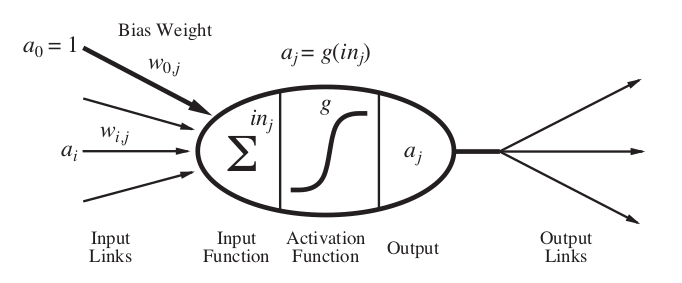
\includegraphics[width=0.8\linewidth]{img/perceptron.png}
	\caption{Model of the perceptron, taken from \cite[]{russell2016artificial}.}
    \label{fig:perceptron}
\end{figure}

A neural network is a collection of many of such neuron components, often layered. The properties of the neurons as well
as the overall network properties are called \emph{hyperparameters} and describe the overall architecture of the \ac{NN}.

A common architecture is the \emph{feed-forward network} which holds several layers of sets of neurons. Each set has no
connection within itself but its activation output is fed into the next layers neurons. It is therefore a directed
acyclic graph. Other than the weights, this network has no internal state and can therefore not hold information about
the input in some form of memory. An alternative is a \emph{\acl {RNN} } which includes loops and therefore can
hold state. The former network is often used for image classification problems while the latter is used for
time-series analysis and natural language processing.

When looking at \ac {NN} one important decision is the number of layers. In fact, the history of \acl{NN} has shown
three key phases of progress, the first phase which included simple single-layer networks, the second which included one
\emph{hidden layer} and the third phase, today, which uses networks that benefit of several hidden layers. A hidden
layer is a number of neurons between the input layer and the output layer. This allows the network to generate complex
input-output relationships. Such a multi-layer network is conceptualized in Figure~\ref{fig:multilayernn}. Each layer
$h^n$ feeds into the next until finally the output layer is reached. 

\begin{figure}[]
    \centering
    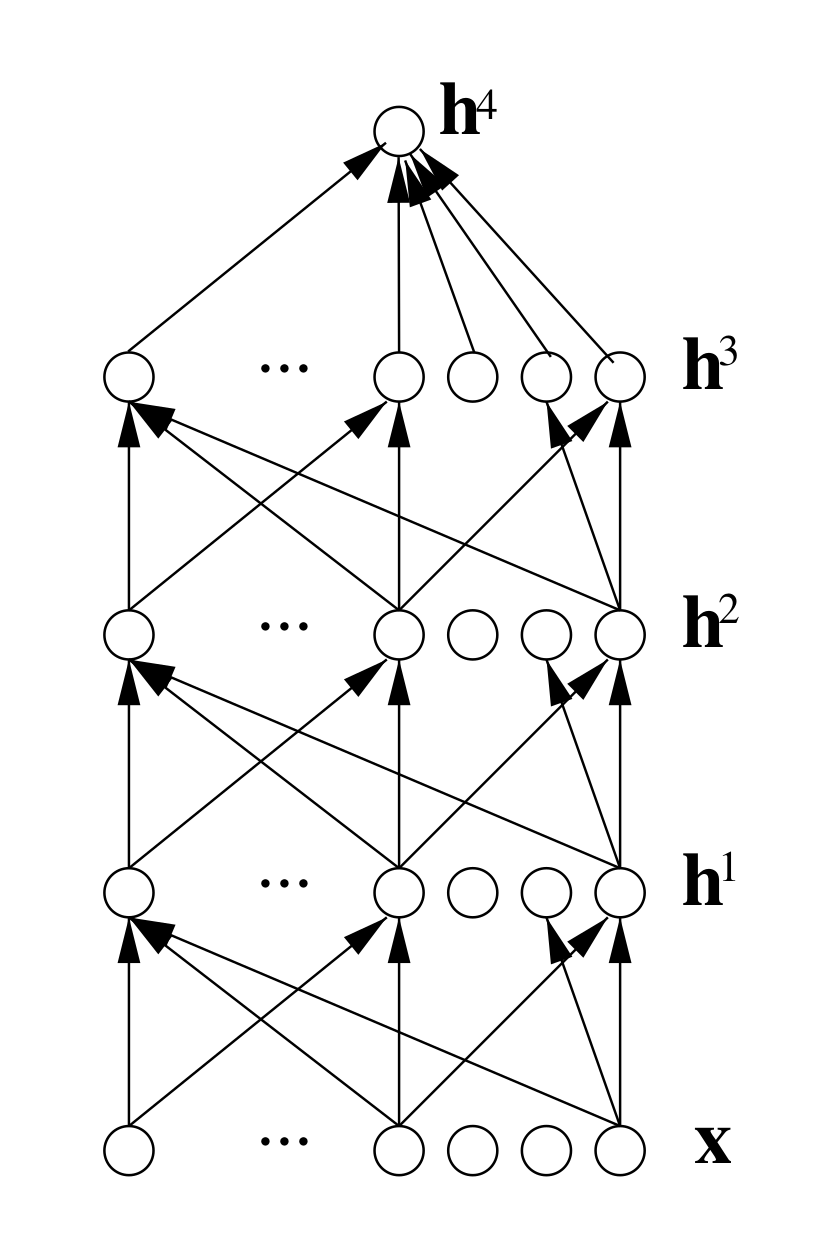
\includegraphics[width=0.3\linewidth]{img/multilayer_nn.png}
	\caption{Multi-layer neural network from \cite[]{bengio2009learning} }
    \label{fig:multilayernn}
\end{figure}

Neural networks can therefore represent complex non-linear and discontinuous functions
\cite[p.732]{russell2016artificial} even with small numbers of layers or neurons. Such \emph{deep} networks however long
suffered from a large issue: It was unclear how to train them, i.e. how to make them learn. The next section describes a
solution to this problem which lead to the latest revolution in \ac {NN} applications. 

